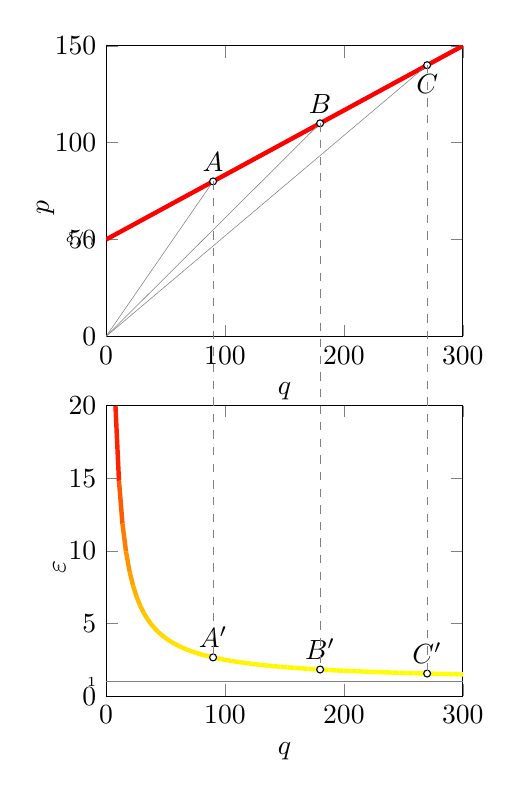
\begin{tikzpicture}
\begin{axis}[
	xmin=0,xmax=300,ymin=0,ymax=150,
height=150pt,
	domain=0:300,
	extra y ticks={50},
	extra y tick style={tickwidth=0},
	extra y tick labels={\tiny{$\delta / \gamma$}},
	xlabel style={below},xlabel=$q$,
	ylabel style={left},ylabel=$p$,
	samples=40]
\addplot[draw=red,ultra thick] {x/3+50};
\node[above] at (axis cs:90,80) {$A$};
\node[above] at (axis cs:180,110) {$B$};
\node[below] at (axis cs:270,140) {$C$};
\addplot[gray,very thin] coordinates {(0,0) (90,80)};	%C: ed=1
\addplot[gray,very thin] coordinates {(0,0) (180,110)};	%C: ed=1
\addplot[gray,very thin] coordinates {(0,0) (270,140)};	%C: ed=1
\addplot[only marks,forget plot,black,mark options={mark size=1.25pt,fill=white},mark=*] coordinates {
	(90,80)	
	(180,110)
	(270,140)};
\coordinate (A) at (axis cs:90,80);
\coordinate (B) at (axis cs:180,110);
\coordinate (C) at (axis cs:270,140);
\end{axis}
\begin{axis}[
	xmin=0,xmax=300,ymin=0,ymax=20,
	yshift=-130pt,
	colormap={bw}{rgb255(0cm)=(255,255,0); rgb255(1cm)=(255,0,0)},
height=150pt,
	extra y ticks={1},
	extra y tick style={tickwidth=0},
	extra y tick labels={\tiny{1}},
	xlabel style={below},xlabel=$q$,
	ylabel style={left},ylabel=$\varepsilon$,
	samples=40]
\addplot[draw=blue,domain=7.9:300,ultra thick,mesh,samples=100] {150/x+1};
\addplot[gray,very thin] coordinates {(0,1) (300,1)};	%C: ed=1
\addplot[only marks,forget plot,black,mark options={mark size=1.25pt,fill=white},mark=*] coordinates {
	(90,2.6667)
	(180,1.8333)
	(270,1.5556)};
\node[above] at (axis cs:90,2.6667) {$A'$};
\node[above] at (axis cs:180,1.8333) {$B'$};
\node[above] at (axis cs:270,1.5556) {$C'$};
\coordinate (AN) at (axis cs:90,2.6667);
\coordinate (BN) at (axis cs:180,1.8333);
\coordinate (CN) at (axis cs:270,1.5556);
\end{axis}
\draw[gray,very thin,dashed] (A) -- (AN);
\draw[gray,very thin,dashed] (B) -- (BN);
\draw[gray,very thin,dashed] (C) -- (CN);
\end{tikzpicture}